%%%%%%%%%%%%%%%%%%%%%%%%%%%%%%%%%%%%%%%%%
% a0poster Portrait Poster
% LaTeX Template
% Version 1.0 (22/06/13)
%
% The a0poster class was created by:
% Gerlinde Kettl and Matthias Weiser (tex@kettl.de)
%
% This template has been downloaded from:
% http://www.LaTeXTemplates.com
%
% License:
% CC BY-NC-SA 3.0 (http://creativecommons.org/licenses/by-nc-sa/3.0/)
%
%%%%%%%%%%%%%%%%%%%%%%%%%%%%%%%%%%%%%%%%%

%----------------------------------------------------------------------------------------
%	PACKAGES AND OTHER DOCUMENT CONFIGURATIONS
%----------------------------------------------------------------------------------------

\documentclass[a0,portrait,15pt]{a0poster}

\usepackage{multicol} % This is so we can have multiple columns of text side-by-side
\columnsep=100pt % This is the amount of white space between the columns in the poster
\columnseprule=3pt % This is the thickness of the black line between the columns in the poster

\usepackage[svgnames]{xcolor} % Specify colors by their 'svgnames', for a full list of all colors available see here: http://www.latextemplates.com/svgnames-colors

\usepackage{times} % Use the times font
%\usepackage{palatino} % Uncomment to use the Palatino font

\usepackage{graphicx} % Required for including images
\graphicspath{{figures/}} % Location of the graphics files
\usepackage{booktabs} % Top and bottom rules for table
\usepackage[font=small,labelfont=bf]{caption} % Required for specifying captions to tables and figures

\DeclareCaptionFont{myblue}{\color{RoyalBlue}}
\captionsetup{labelfont={myblue,bf}}

\usepackage{amsfonts, amsmath, amsthm, amssymb} % For math fonts, symbols and environments
\usepackage{wrapfig} % Allows wrapping text around tables and figures
\usepackage[position=top]{subfig}
\graphicspath{{figures/}{../paper/figures/}{./}}
\usepackage{tikz,pgf}
\usetikzlibrary{arrows,positioning}

\begin{document}

%----------------------------------------------------------------------------------------
%	POSTER HEADER
%----------------------------------------------------------------------------------------

% The header is divided into two boxes:
% The first is 75% wide and houses the title, subtitle, names, university/organization and contact information
% The second is 25% wide and houses a logo for your university/organization or a photo of you
% The widths of these boxes can be easily edited to accommodate your content as you see fit


\begin{minipage}[b]{0.75\linewidth}
\veryHuge \color{NavyBlue} \textbf{Bandwidth extension of musical audio signals with no side information using dilated convolutional neural networks} \color{Black}\\ % Title
\Huge\textit{}\\[2cm] % Subtitle
\huge \textbf{Mathieu Lagrange, F\'elix Gontier}\\[0.5cm] % Author(s)
\huge LS2N, CNRS, \'Ecole Centrale Nantes\\[0.4cm] % University/organization
\end{minipage}
%
\begin{minipage}[b]{0.25\linewidth}
\includegraphics[width=20cm]{figures/logoLs2n.jpg}\\
\end{minipage}

\vspace{1cm} % A bit of extra whitespace between the header and poster content

%----------------------------------------------------------------------------------------

\begin{multicols}{2} % This is how many columns your poster will be broken into, a portrait poster is generally split into 2 columns

%----------------------------------------------------------------------------------------
%	ABSTRACT
%----------------------------------------------------------------------------------------

\color{Navy} % Navy color for the abstract

\begin{abstract}

The benefit of considering \textbf{stacked graphs}~\cite{Byron2008} to \textbf{display audio} data is studied. Thanks to a careful use of layering of the spectral information, the resulting display is both concise and intuitive. Compared to the spectrogram display, it allows the reader to \textbf{focus} more on the \textbf{temporal aspect of the time/frequency decomposition} while keeping an abstract view of the spectral information.

\textbf{Validation} is done using \textbf{two perceptual experiments} that demonstrate the potential of the approach. The first considers the proposed display to perform an \textbf{identification task of the musical instrument} and the second considers the proposed display to \textbf{evaluate the technical level of a musical performer}. Both experiments show the potential of the display and potential applications scenarios in musical training are discussed.

\end{abstract}

%----------------------------------------------------------------------------------------
%	INTRODUCTION
%----------------------------------------------------------------------------------------

\color{SaddleBrown} % SaddleBrown color for the introduction

\section*{Background}

%----------------------------------------------------------------------------------------
%	OBJECTIVES
%----------------------------------------------------------------------------------------
\color{DarkSlateGray}

\begin{center}
\begin{tabular}{|c|c|c|c|}
\hline
& Attack & Body & Decay \\
\hline
Duration & moderate & non-existent & slow \\
\hline
Frequency  & \multicolumn{3}{c|}{steady low} \\
\hline
Fluctuations  & transient & \multicolumn{2}{c|}{steady-state} \\
\hline
Dynamics  & \multicolumn{3}{c|}{loud to soft} \\
\hline
Duration & \multicolumn{3}{c|}{ $\longleftarrow$ 3 seconds $\longrightarrow$ } \\
\hline
\end{tabular}
\captionof{figure}{ \color{RoyalBlue} Annotation of a church bell from Schafer \cite{Schafer1977}.}
\end{center}\vspace{1cm}

\color{SaddleBrown}

\textbf{Schafer} proposed a notational system that can be considered for describing any kind of sound, be it a unique event or any kind of compound~\cite{Schafer1977}. The main rationale is to split the temporal axis from left to right into \textbf{3 parts} corresponding to the \textit{attack}, \textit{sustain} and \textit{decay}. For each part, its duration, \textbf{frequency} (related to the notion of mass as introduced by Schaeffer), \textbf{fluctuations} (related to the notion of grain as introduced by Schaeffer) and \textbf{dynamics} are displayed from top to bottom. Except for the frequency content that is depicted as a rough spectrogram contour, the other dimensions are described according to a specific alphabet of a few symbols.

\begin{center}\vspace{1cm}
  \begin{minipage}[b]{.4\linewidth}
%\includegraphics[width=\linewidth]{churchBell_waveform}
%\includegraphics[width=\linewidth]{churchBell_spectrum}
  \end{minipage}
\begin{minipage}[b]{.5\linewidth}
%\includegraphics[width=\linewidth]{churchBell_spectrogram}
\end{minipage}
\captionof{figure}{ \color{RoyalBlue} Standard displays of the sound of a church bell: waveform (top left), spectrum (bottom left), and spectrogram (right).}
\end{center}\vspace{1cm}

To display \textbf{time vs. frequency vs. energy of a sound} on a \textbf{two-dimensional plane}, one has to resort to a choice or a \textbf{compromise}. Either timing is emphasized and frequency neglected as in the \textbf{waveform} display or frequency is emphasized  and timing neglected  as in the display of the \textbf{Fourier spectrum}.

A compromise is made by considering time and frequency respectively as horizontal and vertical axes of the two-dimensional plane as with the popular \textbf{spectrogram} \textit{magnitude of the short term Fourier transform}. In such display, the use of a color code conveys information about energy.

\color{DarkSlateGray} % DarkSlateGray color for the rest of the

\section*{Introducing the spectral stack display (Spack)}

\textbf{The spectrogram favors frequency over time} :
\begin{itemize}
  \item
  \item \textbf{temporal dynamics and structure are harder to appreciate}, as the way energy fluctuates in each sub bands has to be reconstructed from the color code
  \item \textbf{enlarging the time resolution quickly blurs the frequency resolution} and may lead to a completely non informative display.
\end{itemize}

In order to mitigate those issues, we propose a alternative display that \textbf{favors time over frequency}, the \textbf{spectral stack display (Spack)}.



\begin{center}\vspace{1cm}
\begin{tikzpicture}[box/.style={draw,rounded corners,text width=8cm,align=center}, node distance=5cm]
\node[box] (a) {Mel scaled magnitude spectrogram};
\node[left=of a,font=\bfseries] (aux1) {} ;
\node (b) [box,right=of a,node distance=10cm] {Stacking};
\node[right=of b,font=\bfseries] (c) {};
\draw[->] (aux1) -- node [above] {Audio} (a);
\draw[->] (a) -- node [above] {} (b);
\draw[->] (b) -- node [above] {spack} (c);
\end{tikzpicture}
\captionof{figure}{ \color{RoyalBlue} Processing chain of the spack display.}
\end{center}\vspace{1cm}

To compute the spack display, a \textbf{mel-scaled magnitude spectrogram} is computed from the audio. To each mel spectral band is assigned a given color code from dark blue (low frequency) to yellow (high frequency). At each time frame, \textbf{the spack display is a stacking of the magnitude values of each mel frequency band}.

\begin{center}\vspace{1cm}
%\includegraphics[width=\linewidth]{churchBell_spack}
\captionof{figure}{ \color{RoyalBlue} Spectral stack display (spack) of the sound of a church bell. The color code conveys nicely the modulation within each frequency band and the overall disappearance of the high frequency range.}
\end{center}\vspace{1cm}

\section*{Task 1: Identifying the musical instrument}

Several tones played by \textbf{four musical instruments: piano, violin, trumpet, and flute} are considered as stimuli. Each instrument is played \textit{mezzo forte} at 5 different pitches: C, D, E, F and G. The test is a \textbf{forced-choice categorization task}. Eight subjects, studying at the Engineering school "Ecole Centrale de Nantes", aged from 24 to 26 years, performed the test.

\section*{Task 2: Assessing the level of a saxophone performance}

\begin{center}
  %\includegraphics[width=.5\linewidth]{christophe_B_3_waveform}%\includegraphics[width=.5\linewidth]{francesco_G_3_waveform} \\
  %\includegraphics[width=.5\linewidth]{christophe_B_3_spectrogram}%\includegraphics[width=.5\linewidth]{francesco_G_3_spectrogram} \\
  %\includegraphics[width=.5\linewidth]{christophe_B_3_spack}%\includegraphics[width=.5\linewidth]{francesco_G_3_spack}
\captionof{figure}{\color{RoyalBlue} Graphical displays of \textit{forte} B tone. Several performance issues can be observed: lack of airflow control at the attack, change of pitch and loudness at 3 seconds and lack of steady airflow during the whole performance.}
\end{center}\vspace{1cm}

The stimuli are \textbf{recorded performances of four saxophone players with a technical level assumed to be high or low (2 low, 2 high)~\cite{robine2006evaluation}}. Each player played several tones at pitch B and G. They were asked to play each note in three different ways: \textit{piano}, \textit{forte} and \textit{crescendo decrescendo}.

The test follows a \textbf{XXY structure, where three performances are shown to the subject, one is at a given level (high or low) and the other two of the other level (low or high)}. 16 subjects, studying at the Engineering school "Ecole Centrale de Nantes", aged from 24 to 28 years performed the test.

\section*{Results}

\begin{center}
%\includegraphics[width=.45\linewidth]{instrumentResults}\hspace{2em}
%\includegraphics[width=.45\linewidth]{levelBox}
\captionof{figure}{\color{RoyalBlue} Performance display on (left) the identification of the musical instrument and (right) on  the detection of the level of the saxophone player: sound (S),  waveform (W), spectrogram (Spe) and spack (Spa).}
\end{center}


\color{SaddleBrown} % SaddleBrown color for the conclusions to make them stand out

\section*{Conclusions}

The \textbf{spack} display conveys nicely the distribution of the energy across time and frequency in a way that is an \textbf{alternative} to the one taken when considering the \textbf{spectrogram}.

Subjects of experiments reported \textbf{ease of understanding} and \textbf{quick access} to important aspects of the sounds.

\color{DarkSlateGray} % Set the color back to DarkSlateGray for the rest of the content

%----------------------------------------------------------------------------------------
%	FORTHCOMING RESEARCH
%----------------------------------------------------------------------------------------

\section*{Forthcoming Research}

Future work will focus on the design of validation tasks for the spack display using a \textbf{wider range of audio data}, namely speech and environmental data.

As the spack display is both \textbf{compact} and \textbf{intuitive}, it can be considered as an inspection tool while practicing a musical instrument in order to \textbf{monitor the control of the nuance and the timbre} while playing.

 %----------------------------------------------------------------------------------------
%	REFERENCES
%----------------------------------------------------------------------------------------

%\nocite{*} % Print all references regardless of whether they were cited in the poster or not
\bibliographystyle{plain} % Plain referencing style
\bibliography{bib} % Use the example bibliography file sample.bib

%----------------------------------------------------------------------------------------
%	ACKNOWLEDGEMENTS
%----------------------------------------------------------------------------------------

\section*{Acknowledgements}


The authors would like to acknowledge support for this project
from ANR project Houle (grant ANR-11-JS03-005-01) and ANR project Cense (grant ANR-16-CE22-0012).

%----------------------------------------------------------------------------------------

\end{multicols}
\end{document}
